\documentclass[sigconf, screen]{acmart}

\AtBeginDocument{%
  \providecommand\BibTeX{{%
    \normalfont B\kern-0.5em{\scshape i\kern-0.25em b}\kern-0.8em\TeX}}}


%%% The following is specific to ESEC/FSE '19-SRC and the paper
%%% 'Efficient Computing in a Safe Environment'
%%% by Michail Loukeris.
%%%
\setcopyright{rightsretained}
\acmPrice{}
\acmDOI{10.1145/3338906.3342491}
\acmYear{2019}
\copyrightyear{2019}
\acmISBN{978-1-4503-5572-8/19/08}
\acmConference[ESEC/FSE '19]{Proceedings of the 27th ACM Joint European Software Engineering Conference and Symposium on the Foundations of Software Engineering}{August 26--30, 2019}{Tallinn, Estonia}
\acmBooktitle{Proceedings of the 27th ACM Joint European Software Engineering Conference and Symposium on the Foundations of Software Engineering (ESEC/FSE '19), August 26--30, 2019, Tallinn, Estonia}

\usepackage{amssymb}
\usepackage{amsmath,amssymb,amsfonts}
\usepackage{algorithmic}
\usepackage{graphicx}
\usepackage{textcomp}
\usepackage{xcolor}
\usepackage{tcolorbox}
\usepackage{threeparttable}
\usepackage{siunitx}
\usepackage{cleveref}
\usepackage{array,multirow,graphicx}
\usepackage{booktabs}
\usepackage{filecontents}
\usepackage{multirow}
\usepackage{color, colortbl}
\usepackage{subfig}
\usepackage{makecell}
\usepackage{lipsum}% http://ctan.org/pkg/lipsum
\usepackage{graphicx}

\begin{document}

\title{Efficient Computing in a Safe Environment}
\titlenote{The research described has been carried out as part of the CROSSMINER Project,
which has received funding from the European Union's Horizon 2020 Research and Innovation 
Programme under grant agreement No. 732223  }
\author{Michail Loukeris}
\orcid{1234-5678-9012}
\affiliation{%
	\institution{Athens University of Economics and Business}
	\city{Athens}
	\country{Greece}
}
\email{loukerismichalis@gmail.com}

\renewcommand{\shortauthors}{M. Loukeris}

\begin{abstract}
Modern computer systems are facing security challenges and thus are forced
to employ various encryption, mitigation mechanisms,
and other measures that affect significantly their performance.
In this study, we aim to identify the energy
and run-time performance implications of Meltdown and Spectre mitigation mechanisms.
To achieve our goal, we experiment on server platform using different test cases.
Our results highlight that request handling and memory operations are noticeably affected
from mitigation mechanisms, both in terms of energy and run-time performance.
\end{abstract}

% The code below is generated by the tool at http://dl.acm.org/ccs.cfm.
% Please copy and paste the code instead of the example below.
%
\begin{CCSXML}
	<ccs2012>
	<concept>
	<concept_id>10002978.10003006</concept_id>
	<concept_desc>Security and privacy~Systems security</concept_desc>
	<concept_significance>500</concept_significance>
	</concept>
	<concept>
	<concept_id>10010583.10010662.10010674</concept_id>
	<concept_desc>Hardware~Power estimation and optimization</concept_desc>
	<concept_significance>500</concept_significance>
	</concept>
	</ccs2012>
\end{CCSXML}

\ccsdesc[500]{Security and privacy~Systems security}
\ccsdesc[500]{Hardware~Power estimation and optimization}
\keywords{energy consumption, security measures, safe environment}
\maketitle

\section{Introduction}
Many mitigation patches and services have been introduced, targeting 
modern processors and kernels to shield them from vulnerabilities.
However, the cost of protection is tightly associated with energy consumption
and run-time performance tax.
Nevertheless, disabling security mechanisms, to achieve performance gains,
is feasible while performing computations in a safe environment such as non-cloud
data center {\it e.g} Backup Data Center.

In this research, we focus to identify the energy and run-time performance
of computer systems by dispensing measures that protect against malicious users
such as Meltdown~\cite{meltdown_2018} and Spectre~\cite{spectre_2019}.
Meltdown and Spectre are security vulnerabilities aimed to steal currently processed
data from modern processors.
Prior works have investigated the Meltdown and Spectre and showed that they can degrade
synthetic and realistic workloads run-time performance
significantly~\cite{spectre_performance_2018, SIJMWGDFT_2018, spectre_meltdown_impact}.
However, protection measures that increase reliability but also guard against 
attacks, such as process separation~\cite{PFH_2003} and array bounds checking~\cite{ACCH_2009},
are retained.

To accomplish our task, we perform an empirical study on
Meltdown and Spectre by utilizing a number of popular benchmarks.
The obtained results highlight the energy and run-time performance impact
of Spectre and Meltdown on different types of benchmarks.

\begin{figure*}
	\subfloat{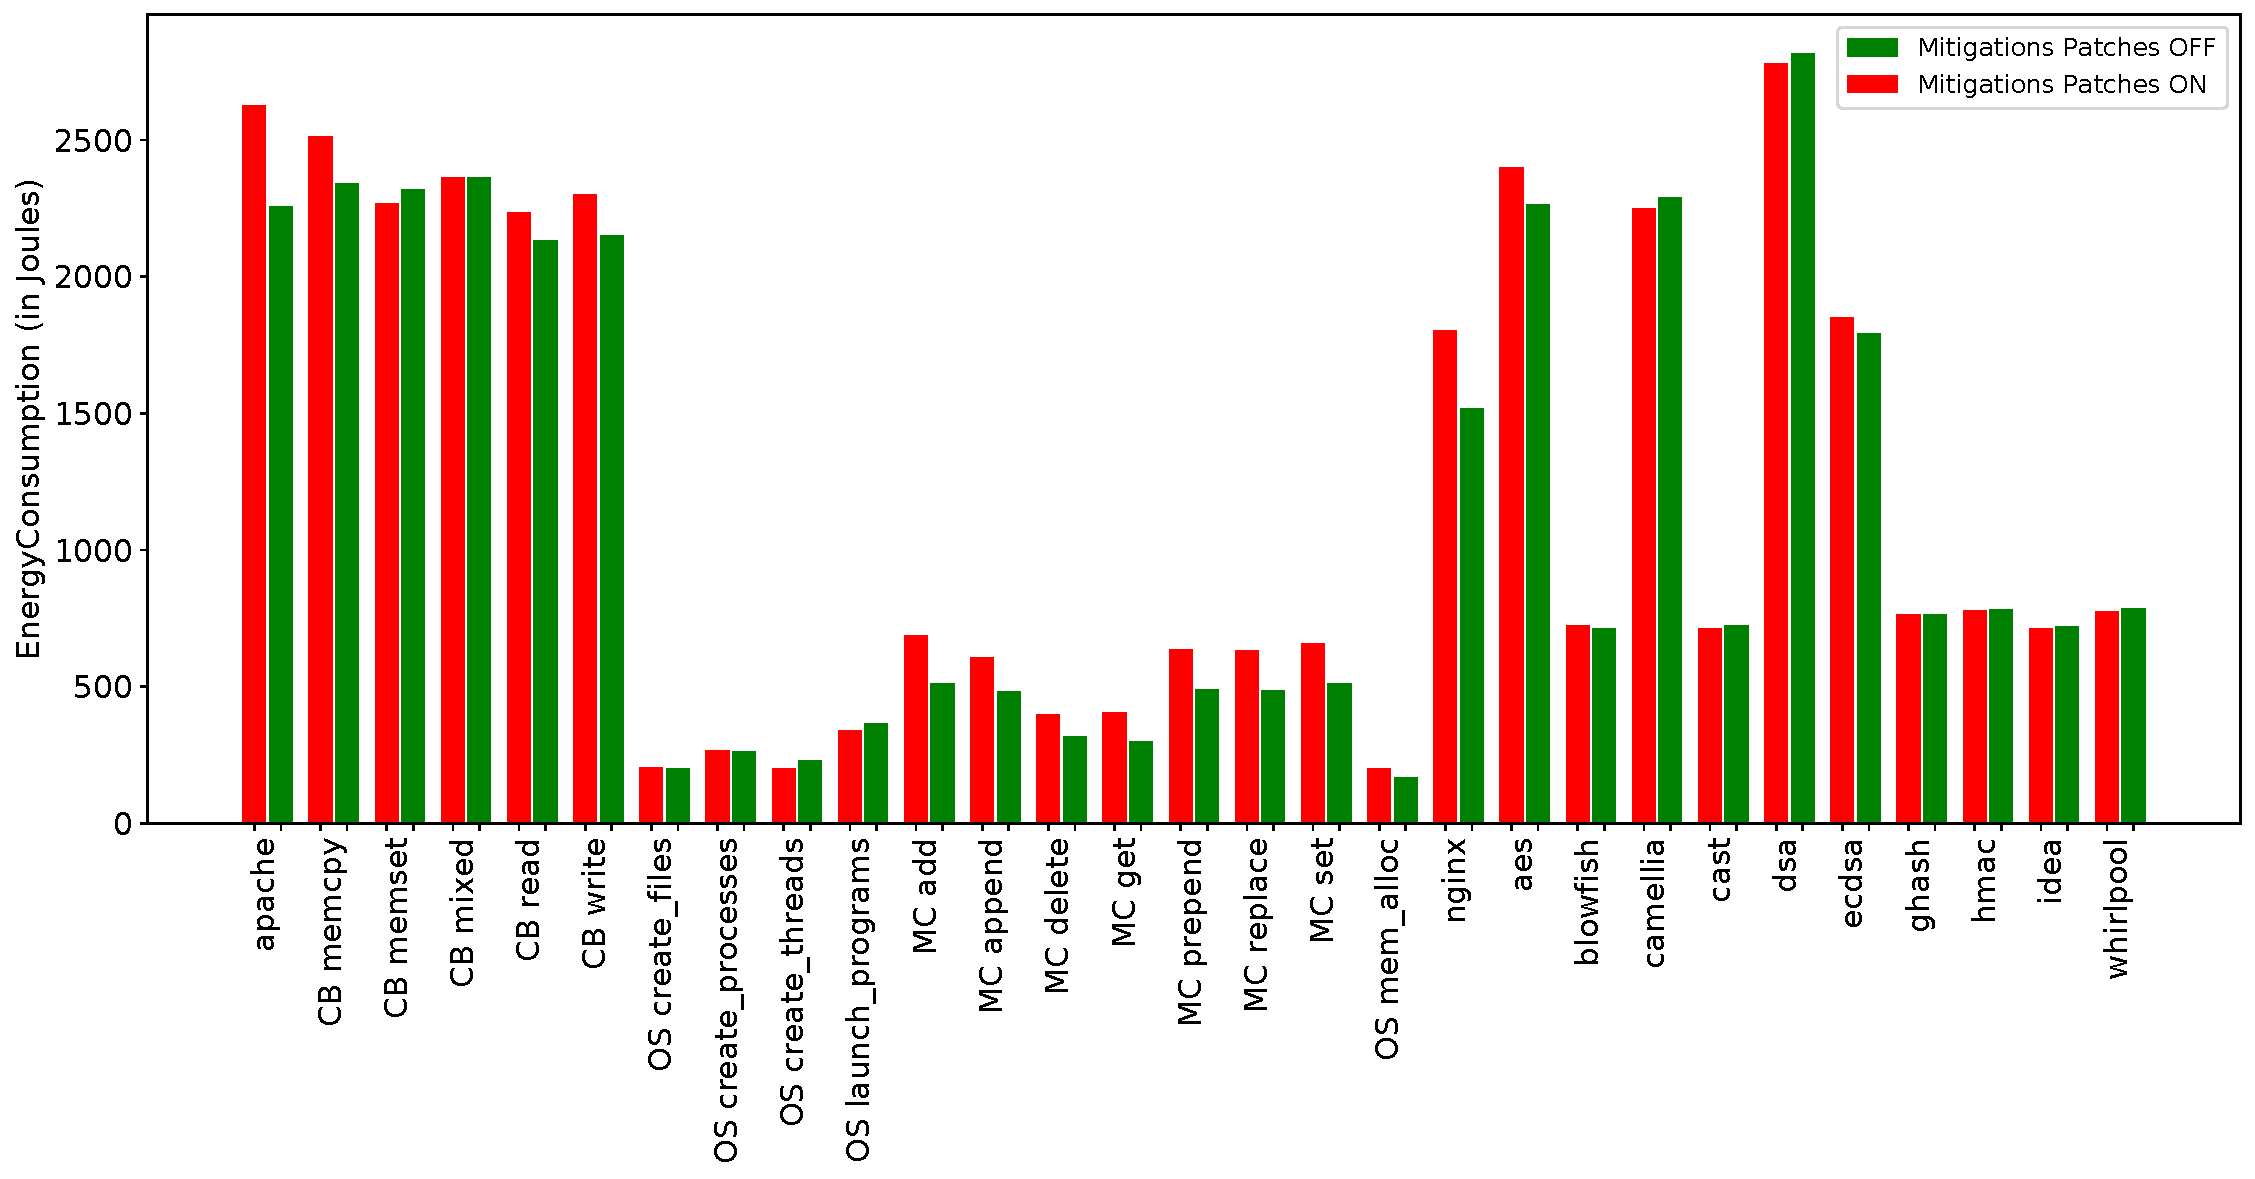
\includegraphics[width=14.40cm,height=5.50cm]{media/energy_results_colored}} \\
	\subfloat{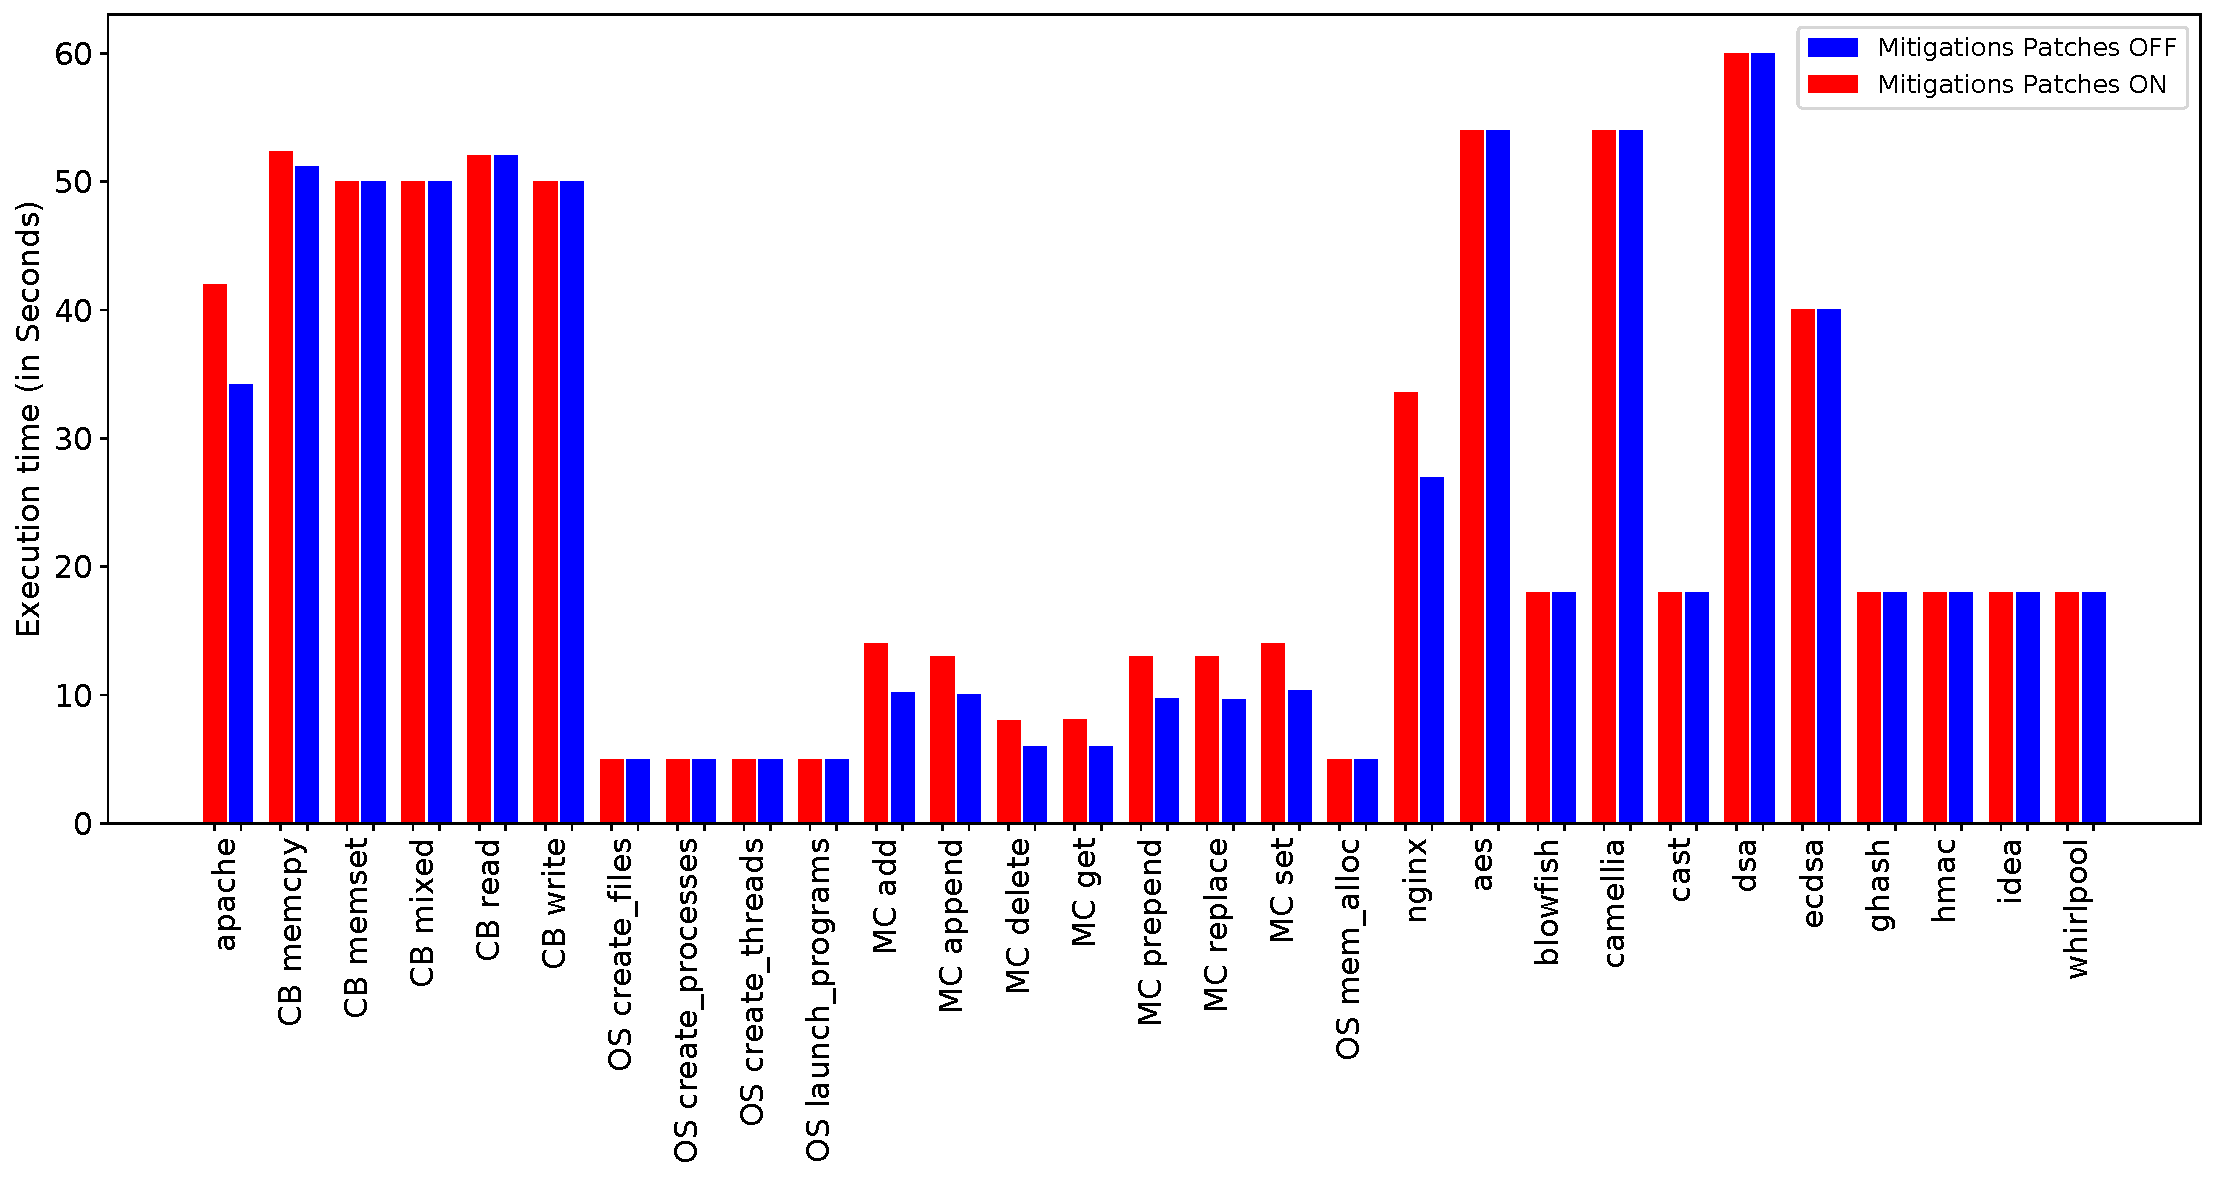
\includegraphics[width=14.40cm,height=5.50cm]{media/performance_colored_results}}
	\caption{Meltdown and Spectre benchmarks energy consumption and execution time}
	\label{fig:energy_run_time_performance_results}
\end{figure*}

\section{Methods}
The goal of our study, is to evaluate the energy and run-time performance
of different security measures to gain understanding over their impact
on various application types.
Therefore, we formulate our research questions as follow:

{\bf RQ1.} {\it What are the energy and run-time performance
implications of Meltdown and Spectre mitigation mechanisms?}\\
\indent {\bf RQ2.} {\it Which application type's energy and run-time performance
	are affected more from Meltdown and Spectre mitigation mechanisms?}

To setup our experiment we used the following subject systems:

{\bf Experimental Platform:}
We performed our experiments on a Lenovo ThinkCentre M910t~\cite{lenovo_thinkcentre}
with Fedora 28 and kernel version 5.0.9-100.
To retrieve energy consumption, we utilized an external device, 
the Watts Up? Pro ({\sc wup})~\cite{watts_up_pro}. 
Also, we used a Raspberry Pi 3B to fetch the energy measurements
from the {\sc wup}'s internal memory via a Linux-based open source utility 
interface~\cite{bailey_watts-up:_2017}. 
We followed this approach to avoid further overhead 
on the computer platform that could affect our energy measurements.

{\bf Test Cases:}
To investigate Spectre and Meltdown, we have selected benchmarks
available from Phoronix~\cite{phoronix_suite}.
Phoronix offers a computer system score by executing
a number of collected, open source benchmarks; however,
without giving the possibility to execute benchmark suites individually.
Therefore, to obtain measurements for our test cases,
we downloaded the desired benchmarks and wrote {\sc bash}
scripts to execute them with the same parameters of Phoronix~\cite{phoronix_github}.
Specifically, we selected benchmarks to examine different functionalities
of a computer system such as
i) {\it Apache~\cite{phoronix_apache} and Nginx~\cite{phoronix_nginx}}
to handle client requests by using {\sc ab} Apache command,
ii) {\it OpenSSL}~\cite{phoronix_openssl} to benchmark cryptographic algorithms,
iii) {\it OSBench}~\cite{phoronix_osbench} to examine operating system primitives such as
creation of file, processes, and threads,
iv) {\it CacheBench}~\cite{phoronix_llcbench} and {\it MCperf}~\cite{phoronix_mcperf}
to investigate cache and main memory operations.

{\bf Running Experiments:}
Before starting our experiment we took a number of precautions to ensure
the validity of our results.
For instance, as suggested by Hindle~\cite{HWRBCR_2014},
we shut down background processes and daemons found in modern
operating systems.
Also, we let a small time window of 30 seconds, between each test case,
to avoid {\it power tails}~\cite{BMM_2012} in our measurements.
Moreover, we executed each test case 20 times to be statistically correct.

\section{Results}
By plotting histograms for each of the benchmarks' test case,
we observed minor variations among their values.
To this end, we decided to depict as results the mean values
of energy consumption and run-time performance.
Figure~\ref{fig:energy_run_time_performance_results}
illustrates the energy consumption in Joules (Top)
and run-time performance impact in seconds (Bottom) of the tasks, respectively.
The Figures X-axis tick labels with acronyms
i) {\sc cb} denotes the {\it CacheBench} tests,
ii) {\sc os} indicates the {\it OSBench} applications,
iii) {\sc mc} shows the {\it MCPerf} tests,
and iv) last ten refer to {\it OpenSSL} cryptograpihc aglorithm test cases.

For {\bf RQ1}, we observe that the results show a significantly higher
energy consumption and run-time performance overhead.
Specifically, mitigation patches of Spectre and Meltdown
may impact energy and run-time performance up to 26\% and 27\%, respectively.
Likewise, for {\bf RQ2} the benchmark types affected the most are
the server benchmarks such as {\it Apache} and {\it Nginx} which were
both affected by high energy consumption and run-time performance overhead.
Moreover, a similar behavior is observed for memory-like operations,
such as {\it memcpy, memset, read, write, add, append, replace, set}
and {\it mem\_alloc}.
At this point, we should mention that the fact most of {\it OpenSSL} benchmarks
don't seem to be affected by the mitigation patches, 
occurs because {\it OpenSSL} collects measurements
of the maximum throughput in a given amount of time.
By examining the cryptographic algorithms throughput without the application of mitigation patches,
we experienced up to 17\% of increased throughput.
Therefore, for the given amount of time and energy, although the measurements
look alike in Figure~\ref{fig:energy_run_time_performance_results},
the cryptographic algorithms without the mitigation patches processed more information.
Moreover, we observe operations such as processes, files, and threads creation
energy consumption where not affected or increased by dispensing the mitigation patches.

\section{Conclusions and Future Work}
In this research, we found out that mitigation patches noticeably affect server systems
and their memory operations, both in terms of energy and run-time performance.
The results are very promising and, therefore, in the future we would like to further
investigate the impact of more security measures such as {\sc tls/ssl}, {\it memory blanking}, 
{\it Zombieload, Fallout} and {\it Ridl} on more computer platforms  in terms of performance
and energy consumption.

As for future work, we aim to develop a requirements-driven adaptive software that takes into
account the type of the application's main operations and switches on/off security measures 
accordingly~\cite{adaptive_security}.


\bibliographystyle{ACM-Reference-Format}
\bibliography{references}
\end{document}
